\subsection{任务一：DDT与LAT的建模及求解}
\label{subsec:lab4-task1}

本任务针对CipherFour的4比特S盒，分别采用one-hot法、逐点排除法、逻辑化简法和凸包法建立混合整数线性规划模型，并枚举各模型的全部二进制解。首先直接计算S盒的DDT和LAT，再以表中的非零位置为参照，检查四种模型得到的输入输出对是否一致。DDT中的$(a,b)$表示输入差分和输出差分，LAT中的$(a,b)$表示输入掩码和输出掩码。% \footnote{本任务的代码实现与报告文字整理使用了AI辅助，实验结果以程序实际运行输出及其与DDT、LAT的核对为依据。}

\paragraph{公共DDT、LAT的计算}

四种方法共用\texttt{ddt\_lat.py}中的表格计算函数。对于DDT，遍历输入差分$a$和输入$x$，计算$S(x)\oplus S(x\oplus a)$，并在对应输出差分的位置累计计数。关键代码如下：
\begin{lstlisting}
for a in range(SIZE):
    for x in range(SIZE):
        b = SBOX[x] ^ SBOX[x ^ a]
        table[a][b] += 1
\end{lstlisting}

对于LAT，遍历输入、输出掩码$a,b$，统计$a\cdot x=b\cdot S(x)$成立的输入个数，再减去8。程序通过按位与和\texttt{bit\_count()}计算模2内积，其核心代码为：
\begin{lstlisting}
equal_count = 0
for x in range(SIZE):
    input_parity = (a & x).bit_count() & 1
    output_parity = (b & SBOX[x]).bit_count() & 1
    if input_parity == output_parity:
        equal_count += 1
table[a][b] = equal_count - SIZE // 2
\end{lstlisting}

运行遍历计算得到图~\ref{fig:lab4-task1-ddt-lat}中的两张表。行下标表示输入，列下标表示输出，均使用十六进制。DDT共有72个非零项，LAT共有122个非零项。因此，差分模型应保留72个合法点，线性模型应保留122个合法点。% LAT中的负值同样表示非零偏差，在提取合法点时使用\texttt{!= 0}判断；两种模型均保留$(0,0)$。

\begin{figure}[H]
    \centering
    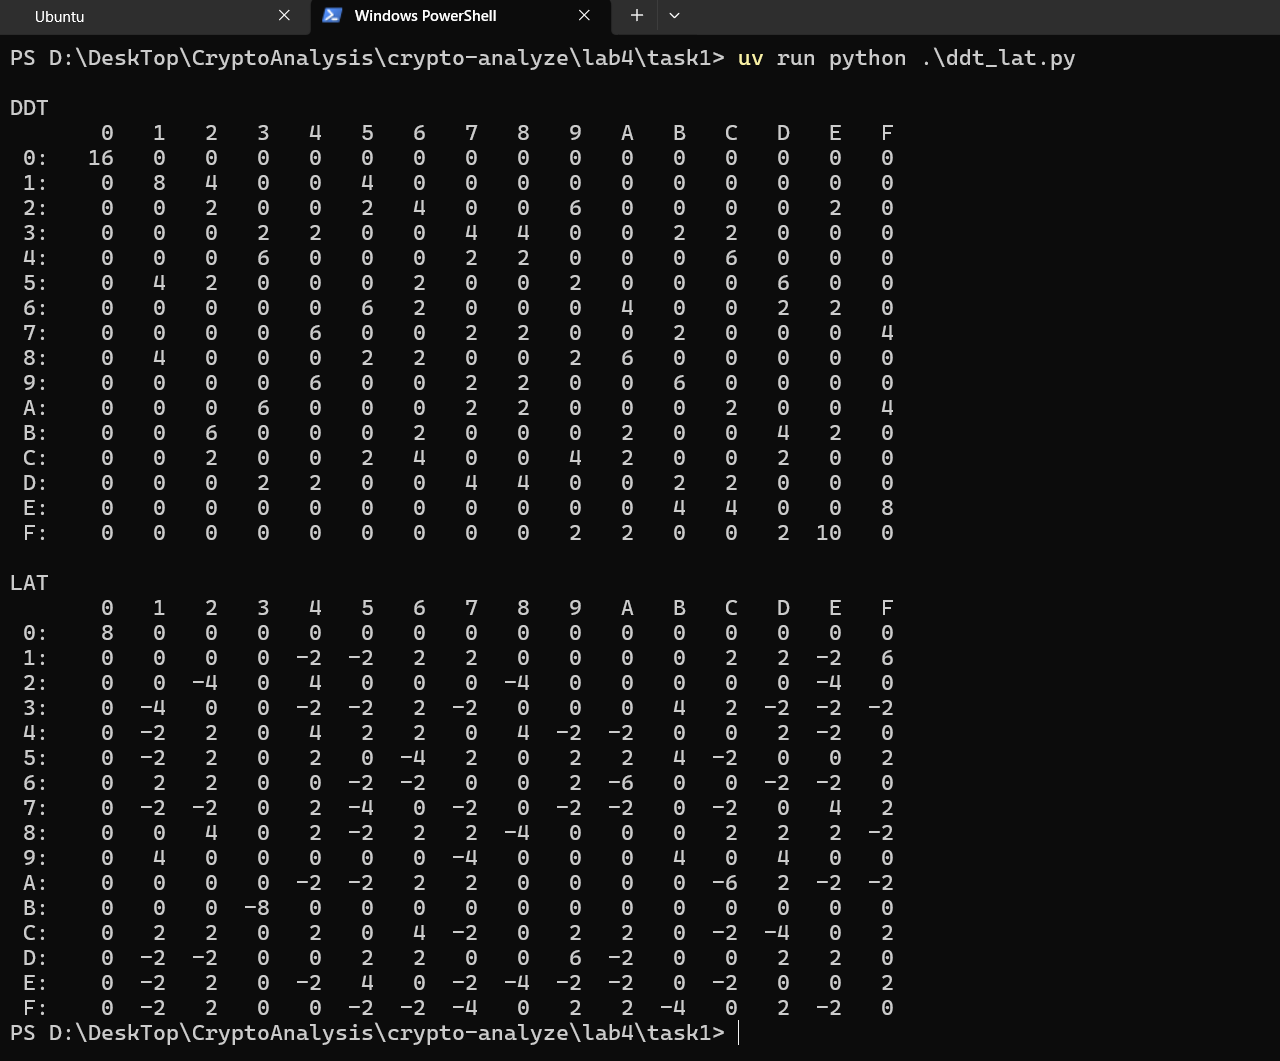
\includegraphics[width=0.90\textwidth]{figures/task1/DDT_LAT.png}
    \caption{直接遍历计算得到的S盒DDT与LAT}
    \label{fig:lab4-task1-ddt-lat}
\end{figure}

\paragraph{统一的编码与枚举方式}

程序将每个输入输出对编码为八位向量
\[
z=(a_3,a_2,a_1,a_0,b_3,b_2,b_1,b_0),
\]
其中输入、输出均按高位在前的顺序排列。四种方法使用相同的位序，以便直接对照求解结果。

为枚举所有合法点，各模型的目标函数均设为常数0，并启用系统性解池搜索：
\begin{lstlisting}
model.setObjective(0, gp.GRB.MINIMIZE)
model.Params.PoolSearchMode = 2
capacity = 2**8 + 1
model.Params.PoolSolutions = capacity
model.Params.MIPGap = 0
model.Params.MIPGapAbs = 0
model.optimize()
\end{lstlisting}

八位坐标共有$2^8=256$种取值，合法点与完整变量赋值一一对应，因此将解池容量设为257。程序在确认求解达到最优且解池未满后，逐个读取解池中的解，按统一位序还原输入输出，并以十六进制排序打印。每个解表示表中的一个非零位置，其具体计数或偏差仍由图~\ref{fig:lab4-task1-ddt-lat}给出。

\clearpage
\subsubsection{one-hot法}
\label{subsubsec:lab4-task1-one-hot}

\paragraph{实验过程与关键代码}

one-hot法从DDT或LAT中提取所有非零位置，组成合法点列表\texttt{points}。随后对每个合法输入输出对设置一个二进制选择变量$\lambda_{a,b}$，并要求所有选择变量之和为1。这样，每次求解都恰好选中一个合法点。

在\texttt{one\_hot.py}中，先用公共函数\texttt{bits(a,b)}保存各合法点的八位编码，再建立8个原始变量和相应的选择变量：
\begin{lstlisting}
points = [(a, b) for a in range(SIZE) for b in range(SIZE)
          if table[a][b] != 0]
point_bits = {point: bits(*point) for point in points}

z = model.addVars(8, vtype=gp.GRB.BINARY, name="z")
lam = model.addVars(points, vtype=gp.GRB.BINARY, name="lambda")
model.addConstr(lam.sum() == 1)
\end{lstlisting}

选择变量确定合法点后，还需要使$z$的每一位等于该点的对应坐标。对于第$j$位，只累加该位为1的合法点所对应的选择变量：
\begin{lstlisting}
for j in range(8):
    model.addConstr(z[j] == gp.quicksum(
        lam[point] for point in points
        if point_bits[point][j] == 1))
\end{lstlisting}

因此，模型包含1条选点等式和8条坐标恢复等式，共9条等式。由于合法点列表中的每个输入输出对互不相同，一组八位坐标也唯一确定被选中的$\lambda$。建立约束后，使用前面的解池参数分别枚举DDT模型与LAT模型。

\paragraph{实验结果与分析}

代码运行结果如图~\ref{fig:lab4-task1-one-hot}所示。
\begin{figure}[H]
    \centering
    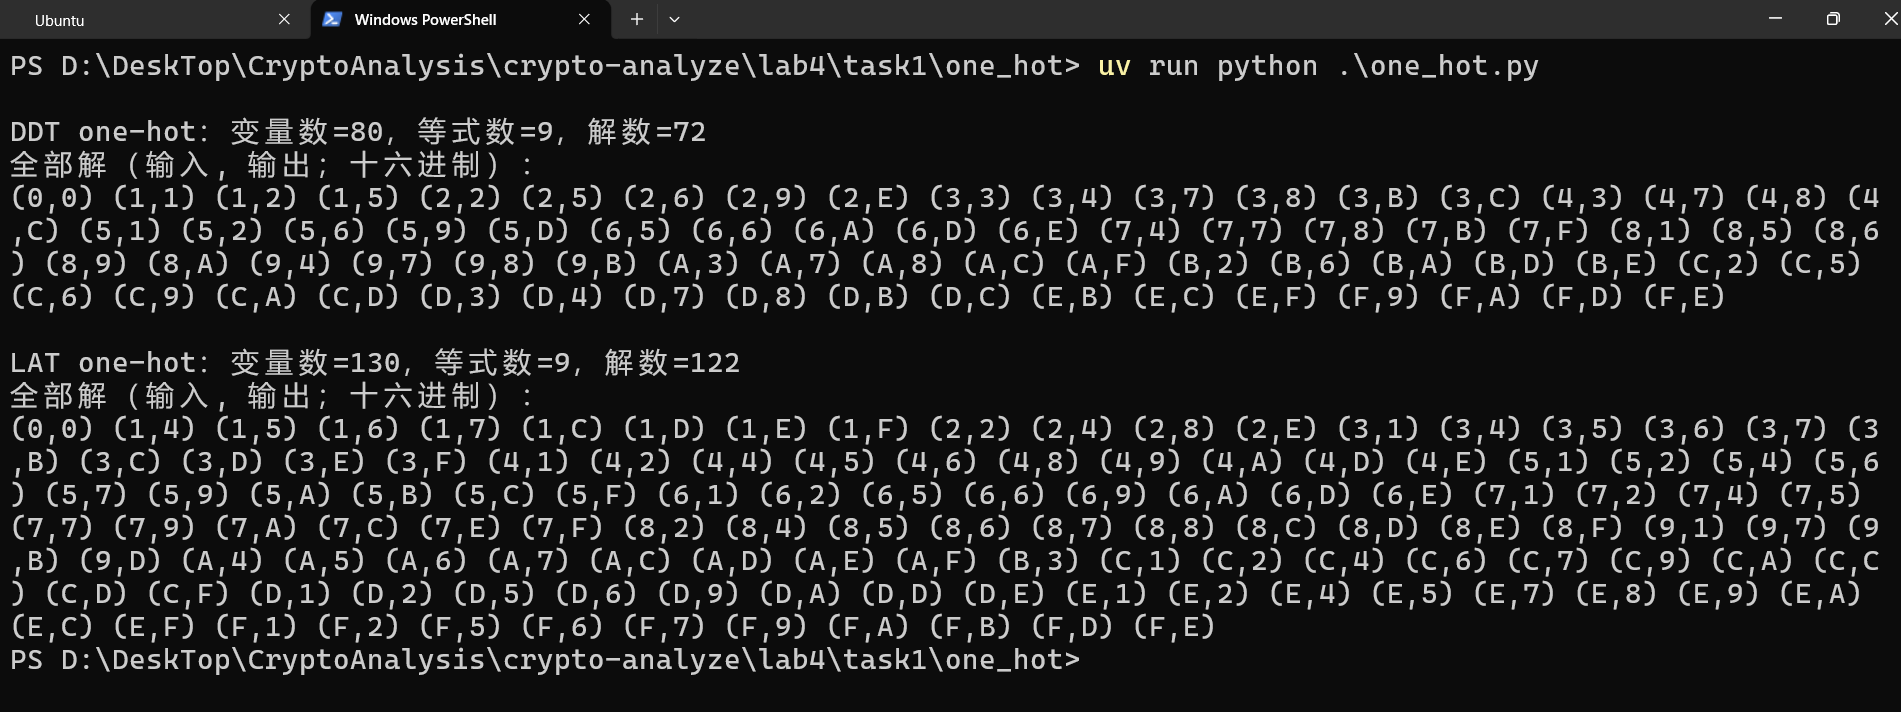
\includegraphics[width=\textwidth]{figures/task1/Grubi_solve1.png}
    \caption{one-hot法的DDT、LAT模型全解枚举结果}
    \label{fig:lab4-task1-one-hot}
\end{figure}

DDT模型有72个选择变量，加上8个原始变量，共$72+8=80$个二进制变量；LAT模型对应$122+8=130$个二进制变量。两者均有9条等式，与上述建模过程一致。求解得到的DDT解数为72，LAT解数为122，按输入分组后与图~\ref{fig:lab4-task1-ddt-lat}各行的非零列逐项相同，说明合法点被完整枚举，零表项对应的点均被排除。

\clearpage
\subsubsection{逐点排除法}
\label{subsubsec:lab4-task1-point-exclusion}

\paragraph{实验过程与关键代码}

逐点排除法先找出表中所有取值为0的位置，组成非法点列表\texttt{forbidden}。模型只设置8个原始二进制变量，然后对每个非法点添加一条排除不等式。由于LAT中正值和负值都属于合法表项，这里统一使用\texttt{table[a][b] == 0}提取非法点。

对于非法点$q$，当$q_j=0$时，$z_j$表示当前点在第$j$位是否与它不同；当$q_j=1$时，则由$1-z_j$表示。因此，将这8项相加并要求结果至少为1，就能保证当前点至少有一位不同于$q$。实现代码如下：
\begin{lstlisting}
forbidden = [(a, b) for a in range(SIZE) for b in range(SIZE)
             if table[a][b] == 0]
z = model.addVars(8, vtype=gp.GRB.BINARY, name="z")

for point in forbidden:
    q = bits(*point)
    model.addConstr(gp.quicksum(
        z[j] if q[j] == 0 else 1 - z[j]
        for j in range(8)
    ) >= 1)
\end{lstlisting}

每条不等式只排除对应的一个非法二进制点。添加全部约束后，剩余可行点就是表中的非零位置，再由Gurobi按统一参数进行枚举。

\paragraph{实验结果与分析}

代码运行结果如图~\ref{fig:lab4-task1-point-exclusion}所示。
\begin{figure}[H]
    \centering
    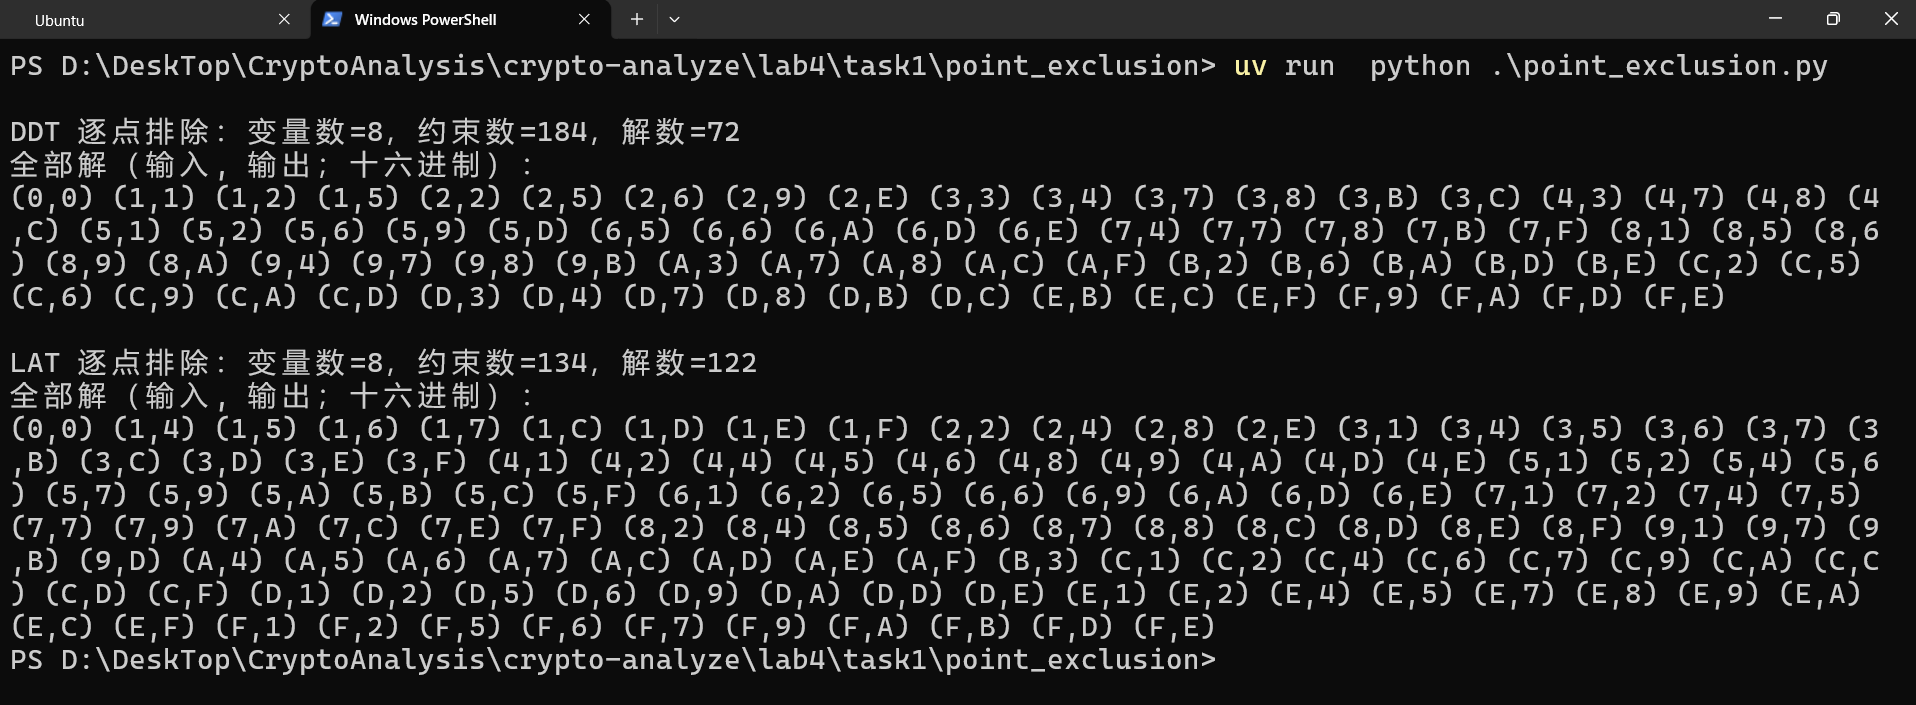
\includegraphics[width=\textwidth]{figures/task1/Grubio_solve_point_exclusion.png}
    \caption{逐点排除法的DDT、LAT模型全解枚举结果}
    \label{fig:lab4-task1-point-exclusion}
\end{figure}

输入、输出各有16种取值，因此共有$16\times16=256$个候选点。DDT中有72个合法点，需要排除$256-72=184$个点，对应184条不等式；LAT中有122个合法点，需要排除$256-122=134$个点，对应134条不等式。两种模型均只有8个二进制变量，与程序输出一致。

枚举得到72个差分合法点和122个线性合法点，具体输入输出对与one-hot法及原始表的非零位置完全一致。该方法保持8个原始变量，通过184条或134条不等式逐点排除非法点，实现了相同的传播关系。

\clearpage
\subsubsection{逻辑化简法}
\label{subsubsec:lab4-task1-logic-minimization}

\paragraph{非法点函数的构造与化简}

逐点排除法中，每个非法点都需要一条不等式。逻辑化简法进一步考虑将多个非法点合并处理：先构造一个八输入布尔函数，使其在非法点上取1，在合法点上取0，再使用Espresso将这个函数化简为若干乘积项。每个乘积项对应一个逻辑立方体，其中部分坐标固定为0或1，其余坐标可以任意取值。

本实验在\texttt{logic\_minimization.py}中通过PyEDA提供的\texttt{espresso\_exprs}接口调用Espresso。\footnote{PyEDA的Espresso接口及两层逻辑化简说明：\url{https://pyeda.readthedocs.io/en/latest/2llm.html}。}程序按公共位序建立8个布尔变量，对每个零值位置生成一个最小项，再将所有最小项取或：
\par\noindent\begin{minipage}{\linewidth}
\begin{lstlisting}
variables = exprvars("x", 8)
minterms = []
for a in range(SIZE):
    for b in range(SIZE):
        if table[a][b] == 0:
            point = bits(a, b)
            minterms.append(And(*(
                variable if value else ~variable
                for variable, value in zip(variables, point)
            )))

forbidden_function = Or(*minterms).to_dnf()
minimized, = espresso_exprs(forbidden_function)
\end{lstlisting}
\end{minipage}\par

化简后的析取范式仍表示同一组非法点。程序从\texttt{minimized.to\_dnf().cover}中逐项读取文字：正文字表示该位固定为1，负文字表示该位固定为0，没有出现的变量用\texttt{None}表示通配位。这里根据文字的唯一标识找到原来的变量下标，使化简前后的坐标始终对应$(a_3,a_2,a_1,a_0,b_3,b_2,b_1,b_0)$。

\paragraph{立方体到线性约束的转换}

对于一个非法立方体，只要当前点有一个固定坐标与它不同，该点就位于立方体之外。因此，对固定为0的位置累加$z_j$，对固定为1的位置累加$1-z_j$，并要求总和至少为1。通配位不参与求和。关键代码为：
\begin{lstlisting}
z = model.addVars(8, vtype=gp.GRB.BINARY, name="z")
for cube in cubes:
    model.addConstr(gp.quicksum(
        z[j] if value == 0 else 1 - z[j]
        for j, value in enumerate(cube) if value is not None
    ) >= 1)
\end{lstlisting}

这样，一条不等式可以排除一个立方体覆盖的多个非法点。Espresso负责构造较紧凑的非法点覆盖，Gurobi负责求解转换后的线性约束，两者在程序中依次执行。模型仍只有8个原始二进制变量。

\clearpage
\paragraph{实验结果与分析}

代码运行结果如图~\ref{fig:lab4-task1-logic-minimization}所示。
\begin{figure}[H]
    \centering
    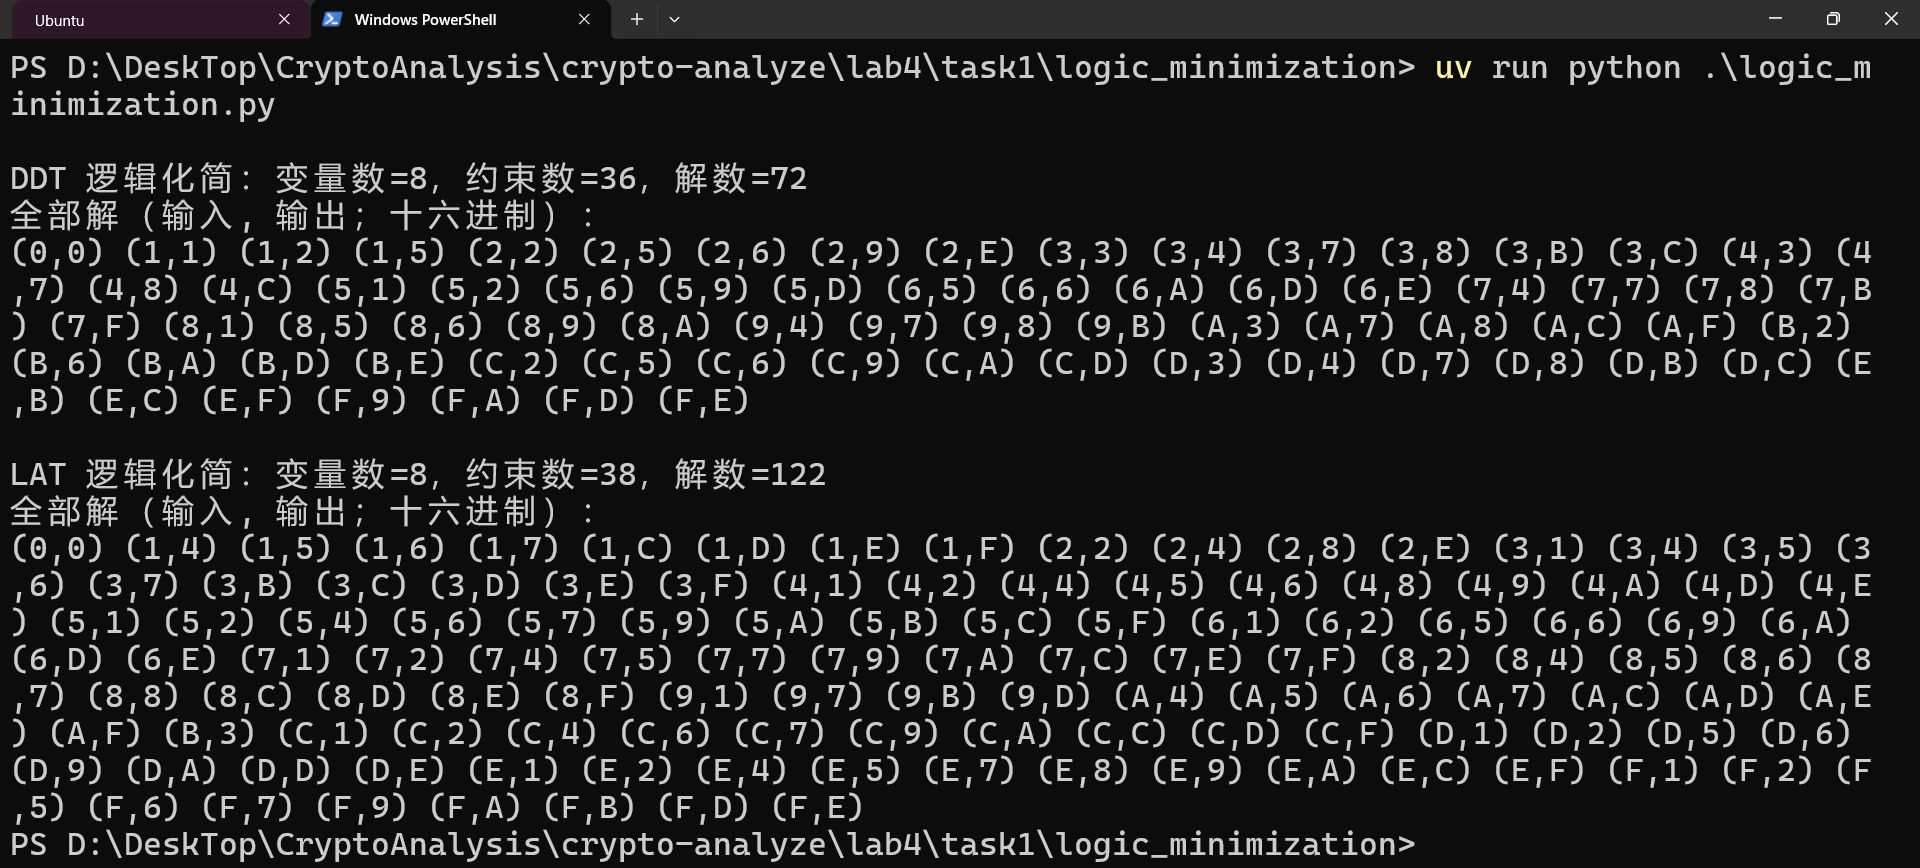
\includegraphics[width=\textwidth]{figures/task1/logistic_minimization.png}
    \caption{Espresso逻辑化简后由Gurobi枚举得到的结果}
    \label{fig:lab4-task1-logic-minimization}
\end{figure}

本次Espresso调用为DDT非法点集生成36个立方体，为LAT非法点集生成38个立方体，因此两个模型分别包含36条和38条不等式。相比逐点排除法的184条和134条，逻辑化简在保留8个变量的同时减少了约束数量。

Gurobi分别枚举出72个差分合法点和122个线性合法点，具体输入输出对与前两种方法一致，也与DDT、LAT中的非零位置一致。这说明立方体合并及其线性约束转换保持了原有的二进制解集。本实验使用的是PyEDA中的Espresso化简接口，36和38记录本次得到的覆盖规模，不能据此认定约束数量已经达到全局最少。

\clearpage
\subsubsection{凸包法}
\label{subsubsec:lab4-task1-convex-hull}

\paragraph{使用SageMath建立完整凸包}

凸包法先从DDT、LAT的非零位置提取合法点，在八维实数空间中构造其凸包，再把凸包的H表示转换成线性约束。实验分为建立凸包和求解两个步骤：\texttt{build\_hull.py}在WSL Arch中使用SageMath计算约束，\texttt{convex\_hull.py}在Windows的\texttt{uv}环境中读取约束并调用Gurobi。

建立凸包时，程序将合法输入输出对编码为八位向量，使用\texttt{QQ}进行精确有理数计算，并分别提取不等式和等式：
\begin{lstlisting}
points = [bits(a, b) for a in range(SIZE) for b in range(SIZE)
          if table[a][b] != 0]
hull = Polyhedron(vertices=points, base_ring=QQ)

hrep = {
    "inequalities": sorted(integer_row(row)
                           for row in hull.inequalities_list()),
    "equations": sorted(integer_row(row)
                        for row in hull.equations_list()),
}
\end{lstlisting}

Sage输出的每行系数按$[c_0,c_1,\ldots,c_8]$排列，第一项为常数，对应$c_0+\sum_{j=0}^{7}c_{j+1}z_j\ge0$，等式使用相同的系数顺序。\footnote{SageMath多面体构造与H表示说明：\url{https://doc.sagemath.org/html/en/reference/discrete_geometry/sage/geometry/polyhedron/constructor.html}。}为便于JSON保存和后续整数计算，\texttt{integer\_row()}先乘以各系数分母的最小公倍数，再约去整数系数的最大公因数。整个过程使用正数缩放，保持不等式方向。

两组完整H表示保存在\texttt{hull\_constraints.json}中，顶层键为\texttt{DDT}和\texttt{LAT}，各自包含\texttt{inequalities}与\texttt{equations}两个系数数组。由于文件位于Windows工作目录，WSL通过\texttt{/mnt/d/}访问并生成文件后，Windows端可以直接读取相同数据。

\paragraph{贪心筛选与Gurobi建模}

完整H表示可以准确描述凸包，但本任务最终只检查二进制点，因此进一步按每条不等式排除非法点的能力进行筛选。程序保留全部等式，将仍满足等式的非法点编号存入\texttt{remaining}，再用\texttt{pool}记录每条候选不等式能够排除的点集。贪心选择的核心循环为：
\par\noindent\begin{minipage}{\linewidth}
\begin{lstlisting}
while remaining:
    row = max(pool, key=lambda item: len(pool[item] & remaining),
              default=None)
    if row is None or not (pool[row] & remaining):
        raise RuntimeError("Incomplete illegal-point coverage")
    chosen.append(row)
    remaining.difference_update(pool.pop(row))
\end{lstlisting}
\end{minipage}\par

其中\texttt{linear\_form(row,point)}计算该行系数在指定点上的值。值小于0表示点违反该不等式，因而可以被排除。候选系数按字典序排列，所以并列时选择顺序固定。每次保留的不等式均来自完整凸包，且筛选结束时所有非法点都已被排除，因此约简后的二进制可行点集仍与原合法点集一致。

最后建立8个二进制变量，将全部等式以$h(z)=0$、筛选后的不等式以$h(z)\ge0$加入Gurobi，再按统一解池设置枚举全部可行点。

\paragraph{实验结果与分析}

SageMath计算完整凸包的输出如图~\ref{fig:lab4-task1-hull-build}所示。
\begin{figure}[H]
    \centering
    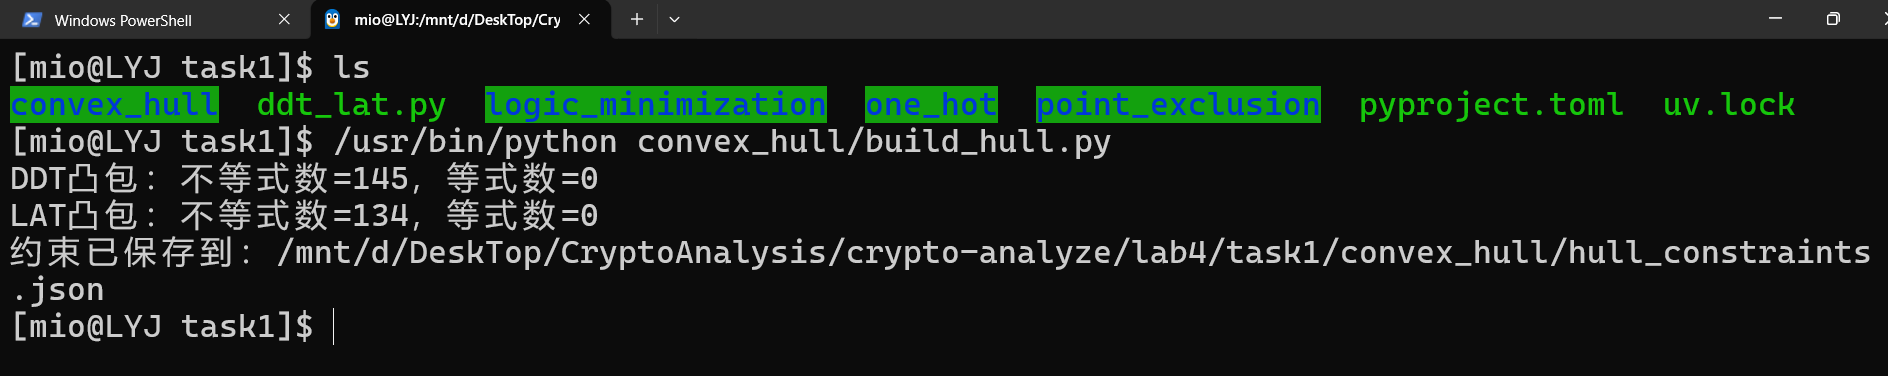
\includegraphics[width=\textwidth]{figures/task1/hell_model.png}
    \caption{SageMath建立DDT、LAT合法点集凸包并保存H表示}
    \label{fig:lab4-task1-hull-build}
\end{figure}

DDT凸包共有145条不等式，LAT凸包共有134条不等式，两者等式数均为0。这与两组合法点集的仿射维数均为8相符。整数化后的约束与直接计算表进行核对时，完整H表示保留的二进制点分别为72个和122个，覆盖全部非零位置。

读取JSON并进行贪心筛选后，Gurobi运行结果如图~\ref{fig:lab4-task1-convex-hull}所示。
\begin{figure}[H]
    \centering
    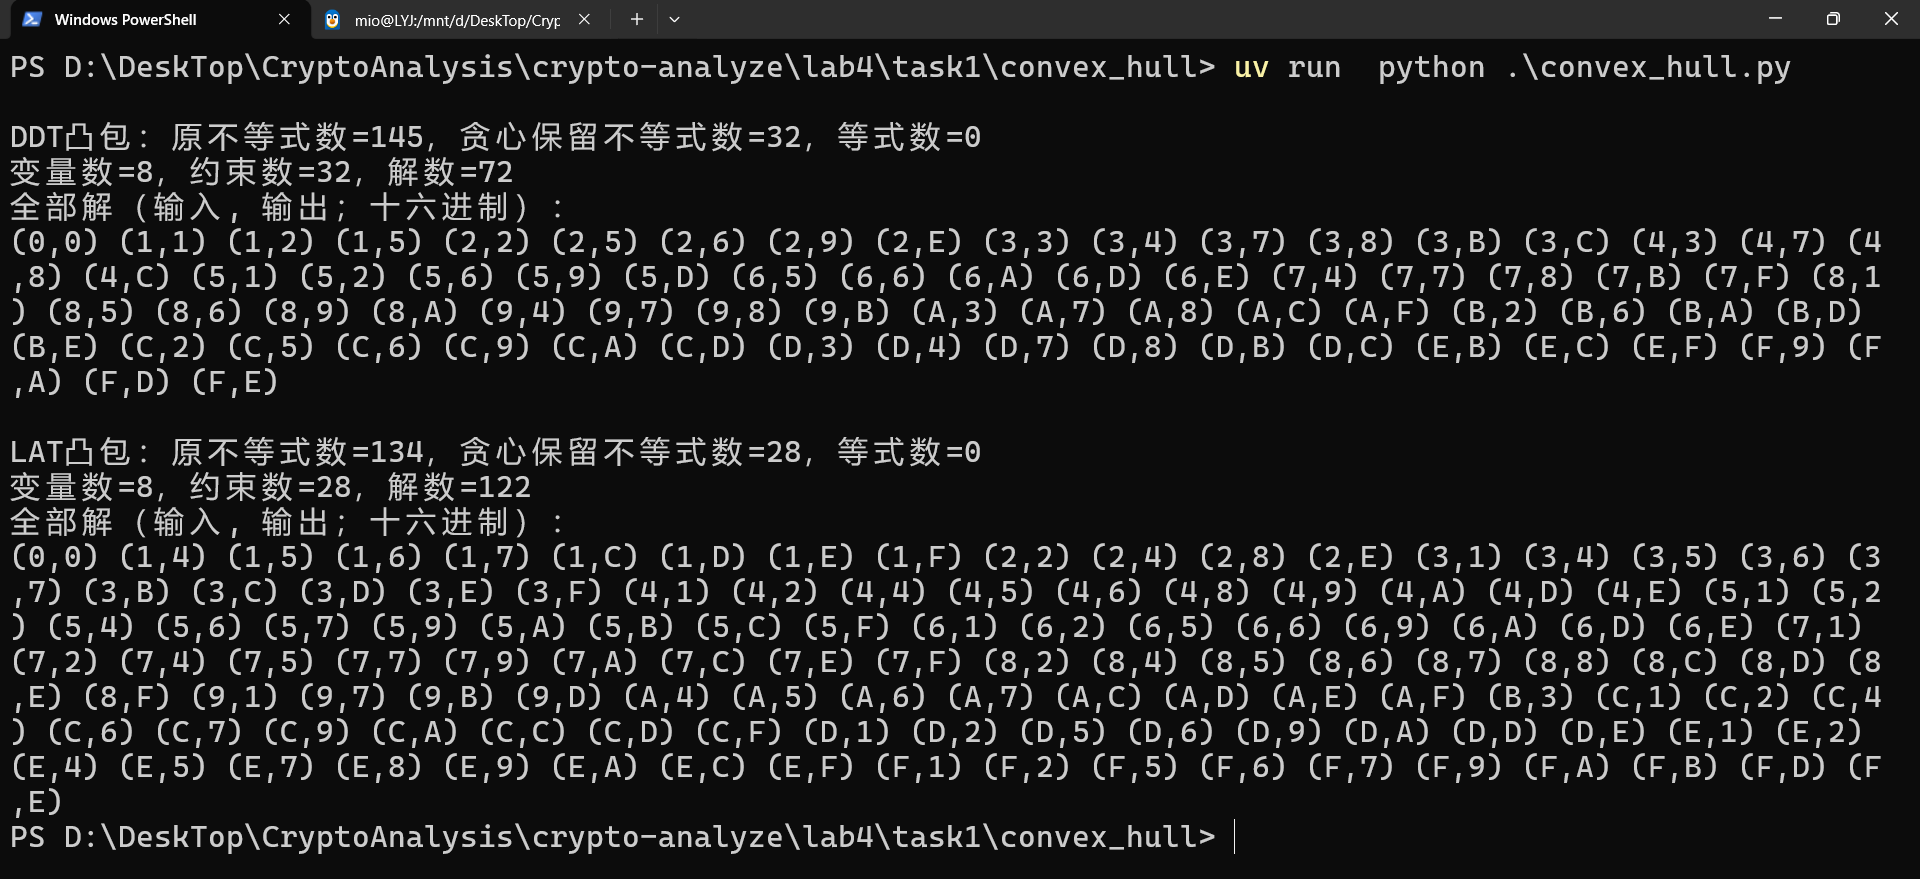
\includegraphics[width=\textwidth]{figures/task1/Grubi_solve3_covex_hell.png}
    \caption{凸包约束经贪心筛选后的Gurobi全解枚举结果}
    \label{fig:lab4-task1-convex-hull}
\end{figure}

DDT模型从145条不等式中保留32条，LAT模型从134条中保留28条。由于没有等式，最终加入Gurobi的约束数分别就是32和28，两种模型的变量数均为8。枚举得到的72个差分输入输出对与122个线性掩码对，与前面三种方法及原始DDT、LAT的非零位置完全一致。

进一步对全部256个二进制点逐一代入约束，完整H表示和筛选后的约束均没有遗漏合法点，也没有保留非法点，说明约束读取、整数化和贪心筛选过程保持了二进制解集。这里的32条和28条约束用于描述合法二进制点；筛选后的连续可行区域可能大于完整凸包，贪心选择也不保证约束数量全局最少。


\clearpage
\subsubsection{四种方法的结果对比}

将四种方法的模型规模和枚举结果汇总，如表~\ref{tab:lab4-task1-comparison}所示。表中的约束数统计显式添加的线性约束，二进制变量的取值范围单独计入变量类型；凸包法使用贪心筛选后实际加入Gurobi的约束数。

\begin{table}[H]
    \centering
    \caption{四种方法的模型规模与全解枚举结果}
    \label{tab:lab4-task1-comparison}
    \begin{tabular}{lrrrrrr}
        \toprule
        \multirow{2}{*}{方法} & \multicolumn{3}{c}{DDT模型} & \multicolumn{3}{c}{LAT模型} \\
        \cmidrule(lr){2-4}\cmidrule(lr){5-7}
        & 变量数 & 约束数 & 解数 & 变量数 & 约束数 & 解数 \\
        \midrule
        one-hot法 & 80 & 9 & 72 & 130 & 9 & 122 \\
        逐点排除法 & 8 & 184 & 72 & 8 & 134 & 122 \\
        逻辑化简法 & 8 & 36 & 72 & 8 & 38 & 122 \\
        凸包法 & 8 & 32 & 72 & 8 & 28 & 122 \\
        \bottomrule
    \end{tabular}
\end{table}

四种方法均准确复现DDT的72个与LAT的122个非零位置，说明二进制解集一致。one-hot法通过增加选择变量减少线性约束条数，其9条约束均为等式；其余三种方法均使用8个变量，其中本次凸包贪心模型的约束数最少。表中反映的是模型规模，约束条数不能直接代替求解时间比较；Espresso化简和贪心筛选的结果也不保证约束数量全局最少。
